%----------------------------------------------------------------------------------------
%	CHAPTER 
%----------------------------------------------------------------------------------------

\chapterimage{chapter_head_2.pdf} % Chapter heading image

\chapter{AGV Manager}

\section{Overview}
AGV Manager have 2 software components: AGV manager it self and AGV configurator.
In AGV configurator are set some parameters like the map file directory, script directory, communication with the AGVs controllers, PLC communication and IO definition, database communication, emulator enabling, etc.

AGV manager will load the parameters set by Agv configurator, and main execute the script written for the specified plant. In AGV manager can be shown the map and motion simulation and modify the script. The script is written in XScript language (Robox scripting language) and executed by AGV manager.

\begin{figure}
	\centering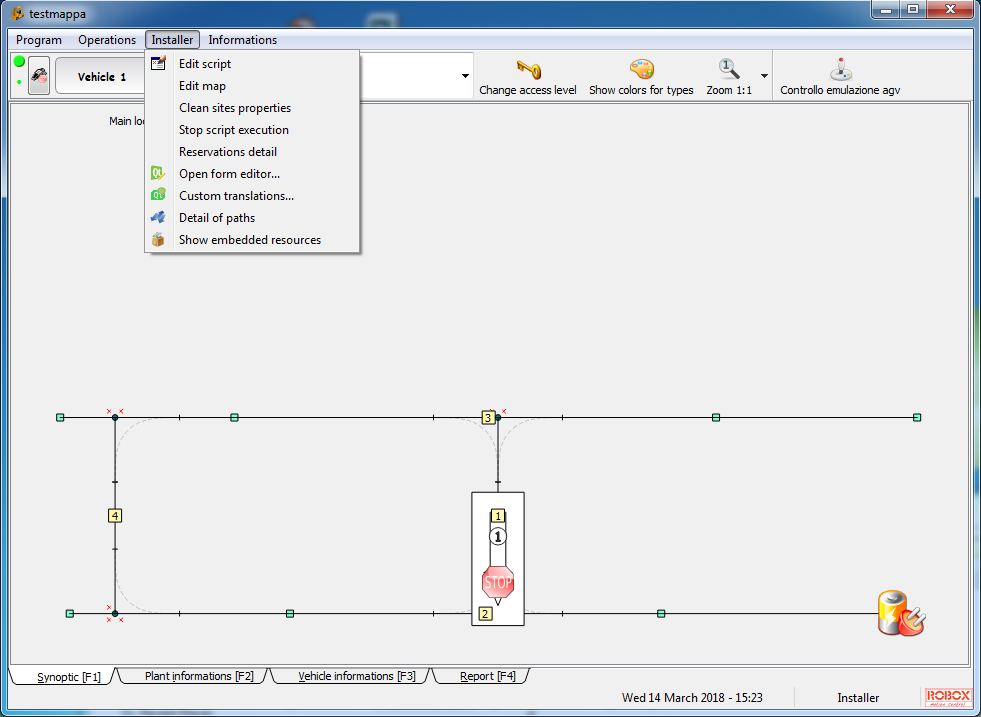
\includegraphics[scale=0.4]{agvmanager/agvManager/agvManagerMain}
	\caption{AGV Manager main window}
	\label{fig:agvManagerMain}
\end{figure}

\section{Installation}
The installation of AgvManger is straightforward, like any program in Microsoft Windows. AgvConfigurator is installed automatically with AgvManager.

In order to get the report from AgvManager a database should be installed. You can install MySql community version.

Once installed, a schortcut to AgvManager and AgvConfigurator have to be done. In the properties of the application, in \textcolor{blue}{Start in} put the location of the folder where your projects are located, fig.\ref{fig:agvappproperties}.

\begin{figure}
	\centering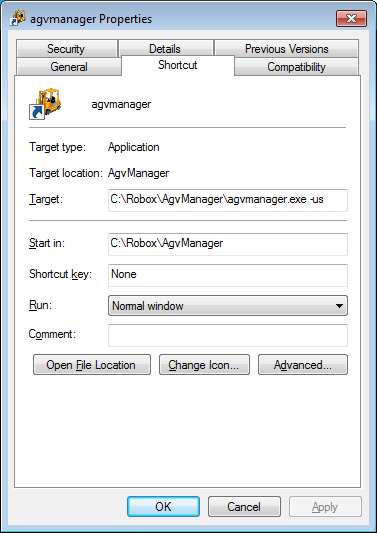
\includegraphics[scale=0.5]{agvmanager/agvManager/agvappproperties}
	\caption{Application properties: Change the "start in" field to your projects directory}
	\label{fig:agvappproperties}
\end{figure}

\section{AGV configurator}

AGV configurator is a standalone program that create a configuration file \textit{.fdoc} for AGV manager. From AgvConfigurator you can select the script to be executed by AgvManager fig.\ref{fig:refConfigScript}, select the map fig.\ref{fig:refConfigMap} and agv \ref{fig:refConfigAgv} and plc communication.

Project folder should be placed in the directory specified in the field \textcolor{blue}{Start in} of the application properties, otherwise it will not work. By default the start point of the application is its installation directory.

The script file should be in the first level of the project folder, it can't be placed in subdirectories, for example \textcolor{red}{appStartDir/Project01/scripts/main.xs} is not allowed, it should be \textcolor{blue}{appStartDir/Project01/main.xs}.

\begin{figure}
	\centering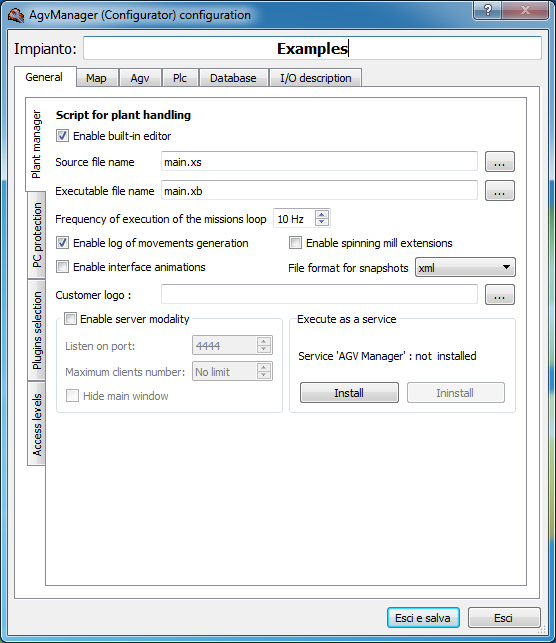
\includegraphics[scale=0.5]{agvmanager/agvManager/agvConfigGeneral1}
	\caption{AGV configurator. General tab, where the \textit{.xs} script file is selected. The script have to be created by an external editor. It is enough to write the name of the executable file with .xb extension, when AgvManager comple the xs file, the xb file will be created automatically.}
	\label{fig:refConfigScript}
\end{figure}
\begin{figure}
	\centering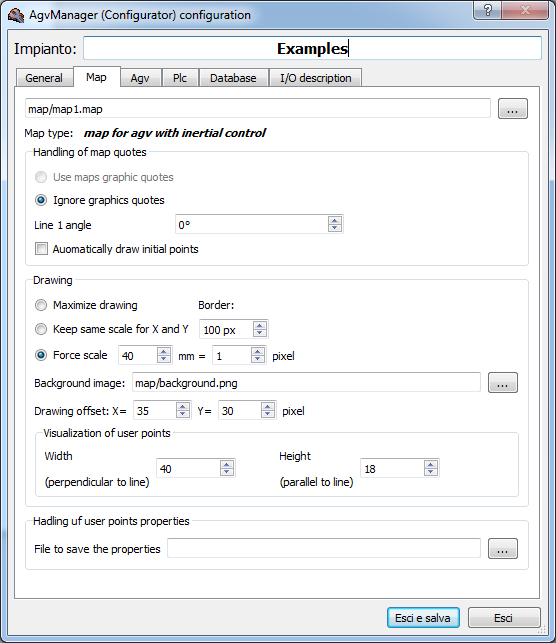
\includegraphics[scale=0.5]{agvmanager/agvManager/agvConfigMap}
	\caption{AGV configurator. Map tab, where the \textit{.map} file is selected. In order to view the user point, you have to set the width and height of it, otherwise user points are not viewed. It is convenient to represent user points as rectangles, not squares.}
	\label{fig:refConfigMap}
\end{figure}
\begin{figure}
	\centering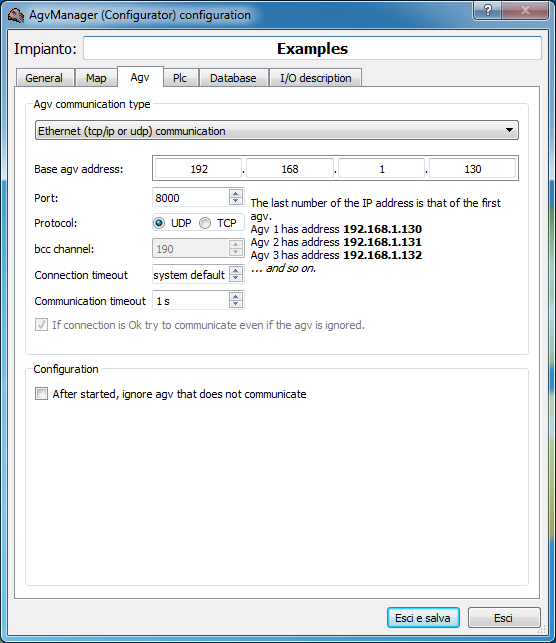
\includegraphics[scale=0.5]{agvmanager/agvManager/agvConfigAgv}
	\caption{AGV configurator. AGV tab, where communication parameter with the AGV are set.}
	\label{fig:refConfigAgv}
\end{figure}

\section{AgvManager interface}
AgvManager have one menu bar, one tool bar, one status bar, map visualization and different tabs [Fx].

In the tool bar, fig.\ref{fig:toolbar}, we can find the button: Vehicle status, Commands insertion, Access level, color type, Zoom, Agv emulation, user define forms.

In the status bar we can see some message from the script, date and time, and current access level.

\begin{figure}
	\centering
\includegraphics[scale=0.5]{agvmanager/agvManager/toolbar}
	\caption{AgvManager tool bar }
	\label{fig:toolbar}
\end{figure}

\subsection{AGV emulation}
If the flag \textit{emuagv.dll emulazione agv} in AgvConfigurator, we can emulate the AGV in AgvManager. The windows of the emulation can be opened via the button \textit{Controllo emulazione agv}.\\

The window in fig.\ref{fig:refAgvEmu} shows the status of the Agv, groupbox \textit{"Stato"}, where are viewed the 32 Vehicle Status flags (XVehicleInfo.uStatus). The first 4 flags are written by the vehicle and the others can be defined by user.
The first 4 bits (flags) are:
\begin{itemize}
	\item Power enabled
	\item Execution command
	\item Charging battery in progress
	\item Load present, or Unit load present
\end{itemize}
These flags correspond to:
\begin{lstlisting}
// Vehicle status flags, bit mask 2^n.
// 4 least significant bits

$define VST_POTENZA_ATTIVA   1 // Power active, mask bit 0
$define VST_EXEC_COMANDO     2 // executing command, mask bit 1
$define VST_CARICA_INCORSO   4 // charge in progress, mask bit 2
$define VST_CARICO_PRESENTE  8 // load present, mask bit 3
\end{lstlisting}

The Battery box, indicate the amount of power consumed, not the remaining one. for example if the status is 100\%, this mean the battery is empty, if the progress bar indicate 20\%, this mean the remaining power is 80\%. The value of the remaining gpower is shown in the \textit{Battery capacity} progress bar in the tab \textit{Vehicle informations [F3]}.\\

To emulate the Agv, first the Agv emulation should be active, state shown in tab Vehicles (Veicoli). Then in the vehicle tab the operating mode can be selected, and the status can be emulated. The Agv should be in automatic and power is enabled in order to move the Agv.
For example, if we set the flag \textit{Load present} to one, the agv behave depending on the script logic. If the load is a loading unit and there is a load in some station to take out, the Agv will go to that station. Or for example if the load is properly the final product the agv may transport it to some unloading station.

\begin{figure}
	\centering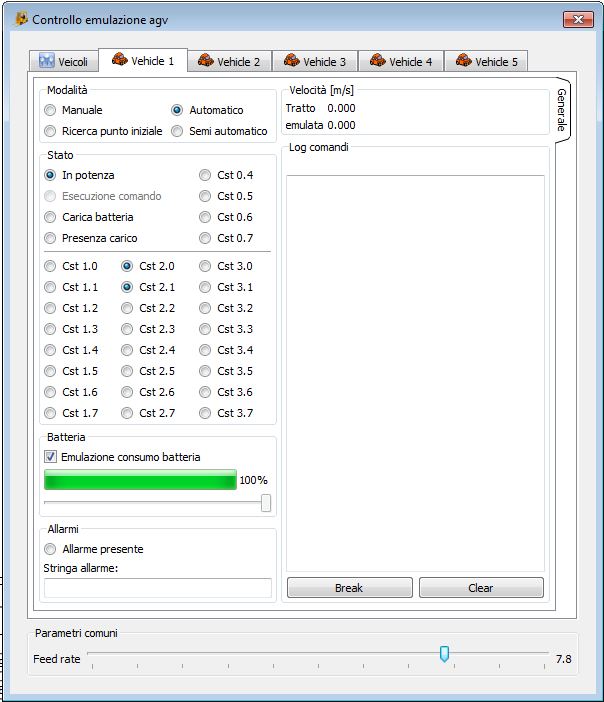
\includegraphics[scale=0.5]{agvmanager/agvManager/agvEmulation}
	\caption{Emulation windows. We can see Agv status flags and other informations. The progress bar indicate the consumed power of the battery, not the remaining power, e.g. 100\% is battery empty. }
	\label{fig:refAgvEmu}
\end{figure}

\subsection{Point windows property}
A user point can be viewed as rectangle, where the dimensions are set in AgvConfigurator. A CBat (Battery point) is shown as a battery icon and . A double click on a user point or battery point a window is opened, see fig.\ref{fig:refLocation}.

In the tab Storage informations, fig.\ref{fig:refLocStorageInfo}, changing the type we can see the description associated to is, e.g. Type 1 is an empty trolley. The spin box (numeric updown control) is used to show only the type, the type is a combination of the checkboxes.

Properties assigned by the function \textit{AddIntProperty()}, are shown in the tab Properties fig.\ref{fig:refLocationProperties}.

\begin{figure}[h]
	\centering
	\begin{subfigure}[b]{0.5\textwidth}
		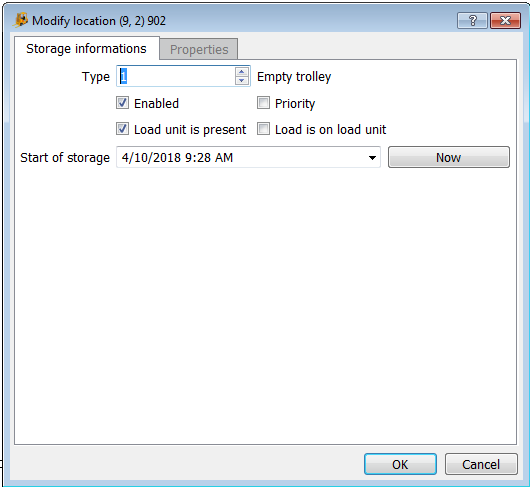
\includegraphics[width=\textwidth]{agvmanager/agvManager/locStorageInfo}
		\caption{Storage information: Load information are shown, timestamp of loading, load type.}
		\label{fig:refLocStorageInfo}
	\end{subfigure}
	\quad
	\begin{subfigure}[b]{0.5\textwidth}
		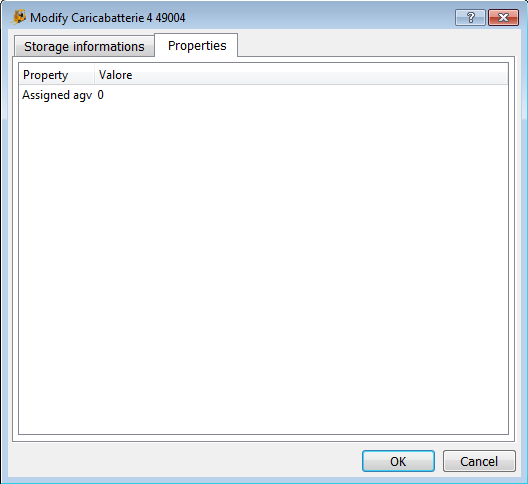
\includegraphics[width=\textwidth]{agvmanager/agvManager/locProperty}
		\caption{Location properties}
		\label{fig:refLocationProperties}
	\end{subfigure}
	\caption{Location window: Storage information and properties}\label{fig:refLocation}
\end{figure}

\section{AGV script executing}
AGV manager can be compared to a plc (hardware and firmware) and the script to a plc program. The firmware is the same in all plant (beside updates and new functionality) and the script change from plant to another.

AGV scripts are written in Xscript language. Xscript have some OOP properties (creating classes and objects), some event handling (mouse move event) and callback functions.

%\newpage
\subsection{Fundamental concepts}
Callback functions are called automatically by AgvManager. A list of callback functions can be found in the documentation \textit{x-script interface, Modules, Estensione x-script per AgvManager, Functions called by AgvManager (callbacks)}.

For example the callback function \textit{OnApplicationStart() : bool} is called once, at the first execution of the script, and the function \textit{OnApplicationStop() : bool} is called when the script execution is stopped.

An example of mouse event handling is the function \textit{onAgvDroppedToPoint (uint uagv, uint upointid, uint orientation)}.
When the agv is dragged and dropped to a point, agv manager call automatically the function onAgvDroppedToPoint() and the code implemented will be executed. As input parameters, the agv index (agv 1 have index 0), destination point and orientation are passed.

In the following section we will se when other callback function are called by AgvManager.\\

Some variable definitions (using \#define keyword) can be found in the documentation \textit{x-script interface, Modules, Estensione x-script per AgvManager, Funzioni per la gestione degli agv}. For example the AGV operative modes can be find with the prefix "MOD\_ ", i.e. MOD\_AUTOMATICO.\\

The following concepts have to be understood before proceeding: Mission, MACRO, MICRO and operations.

Let's say a vehicle have to go from $P_{1}$ to $P_{2}$. This can be considered a mission. A Mission is started by calling \textit{agvStartMission(agv id, missionCode, mission description)} and terminated by calling \textit{agvStopMission(agv id)}.

A mission can be composed from different MACROs. Let's say a MACRO is a macro operation that subdivide the mission. For example our mission can have 3 different MACROs. If the AGV is charging the battery, we have to stop charging (if the energy is enough to execute the whole mission), move to destination, communicate the end of the mission.

Using the 2 defined constants by AgvManager our mission is composed from : MAC\_CHARGE\_STOP, MAC\_END and another macro that we can define using the \$define keyword MAC\_MOVE\_TO\_P.
It is better to define our constants from 100 to avoid errors in the program logic. For example if the already defined constant MAC\_END have value 10, and our constant MAC\_MOVE\_TO\_P have value 10, the compiler will not give errors and the agv will behave as is not expected.

AgvManager have in memory a list(array) of the MACROs to be executed. In the list are saved the agv number/id, MACRO code/id and other 4 parameters. 
When the function 
\textit{agvaddmacro	(	uint 	uagv,
	uint 	ucode,
	int 	ipar1 = 0,
	int 	ipar2 = 0,
	int 	ipar3 = 0,
	int 	ipar4 = 0 
	)		} 
is called, the new MACRO is queued at the end of the list.

A MACRO is composed from MICROs. Let's say, low level micro instructions to be executed by the AGV. There are different types of MICRO, can be found in the constant defintions with prefix MIC\_. For example MIC\_MOVE is a MICRO that handle the motion instruction to the AGV.

A micro is registered (ask to be executed) by calling AgvRegisterSystemBloccante, agvRegisterSystemPassante or AgvRegisterOperation.

An operation is a type of MICRO, a typical kind of operations are loading and unloading, and can be performed on user points.
More about MICRO and operations later and the commands sent to the agv in order to execute orders from AgvManager. Remember that not all MIC instruction send commands to the agv. 

\subsection{Main loop execution}
The following is a simplified explanation of the main loop of and AGV script, which is in execution behind the scene. A more complex scenario is shown in fig.\ref{fig:mainLoop}.
When the script is executed the first time, the function \textcolor{blue}{OnApplicationStart()} is called. In this function you can initialize some variables and set some parameters. After that AgvManager wait for events e.g. mouse events, or operating mode change. And continue to execute some other functions.

In the case we have more than one Agv, the execution of the functions is sequential. This mean that the set of functions of Agv 1 are called first, then those of Agv 2, then Agv 3, etc. In other words, the flowchart in fig.\ref{fig:mainLoop} and fig.\ref{fig:missionExec} are executed starting from the first Agv until the last in sequence, this flow is repeated always.

Let's see a simple case. The AGV is in automatic mode \textcolor{blue}{(MOD\_AUTOMATIC)}, and there is no mission in progress. If the AGV is enabled, AgvManager call automatically the callback function \textcolor{blue}{onNextMission()}, where the programmer have implemented a logic to register the next mission to be executed. When a mission is in progress, AgvManager wait (wait doesn't mean stop script execution) till the end of the mission in order to call again \textcolor{blue}{onNextMission()}.

\begin{figure}
	\centering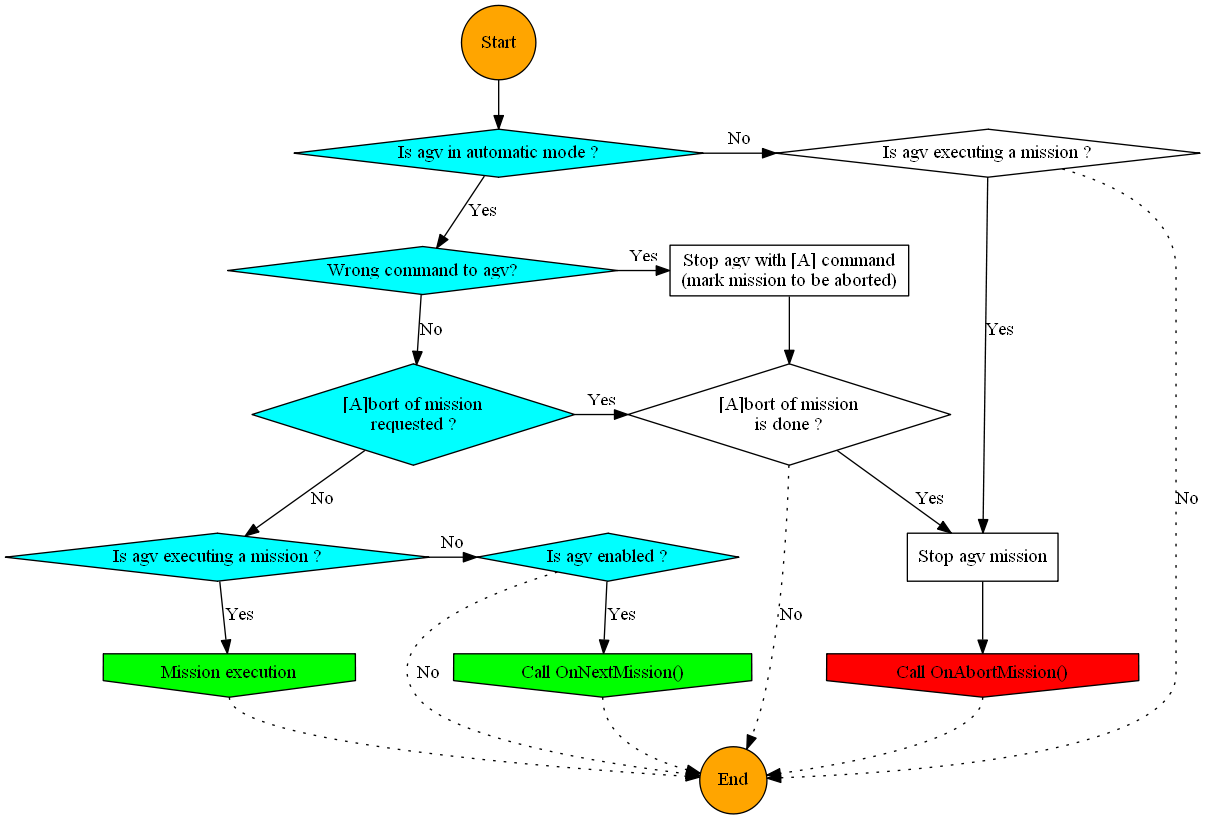
\includegraphics[scale=0.5]{agvmanager/mainloop}
	\caption{Main loop execution}
	\label{fig:mainLoop}
\end{figure}

\subsection{Mission execution}
A mission is a set of MACROs. There is a list of MACROs, where the order of execution is assigned.
A mission can be assigned by a call to \textcolor{blue}{onNextMission()}, and started by calling \textcolor{blue}{AgvStartMission()}.
If the list of MACROs is not empty, the effective execution of the mission begin otherwise the old MICRO continue to execute until the end.

We take only one case, if the MACRO list is not empty, the function \textcolor{blue}{onExpandMacro()} is called by AgvManager.
Then \textcolor{blue}{onExecuteMicro()} is called. At the last call of \textcolor{blue}{onExecuteMicro()} the paramater \textcolor{blue}{bLastCall} is assigned to true.

Fig.\ref{fig:missionExec} show a flow chart about the mission execution.
That is a single step of the mission. We have to imagine that AgvManager continue to call the flowchart like a plc, cyclically.

\begin{figure}
	\centering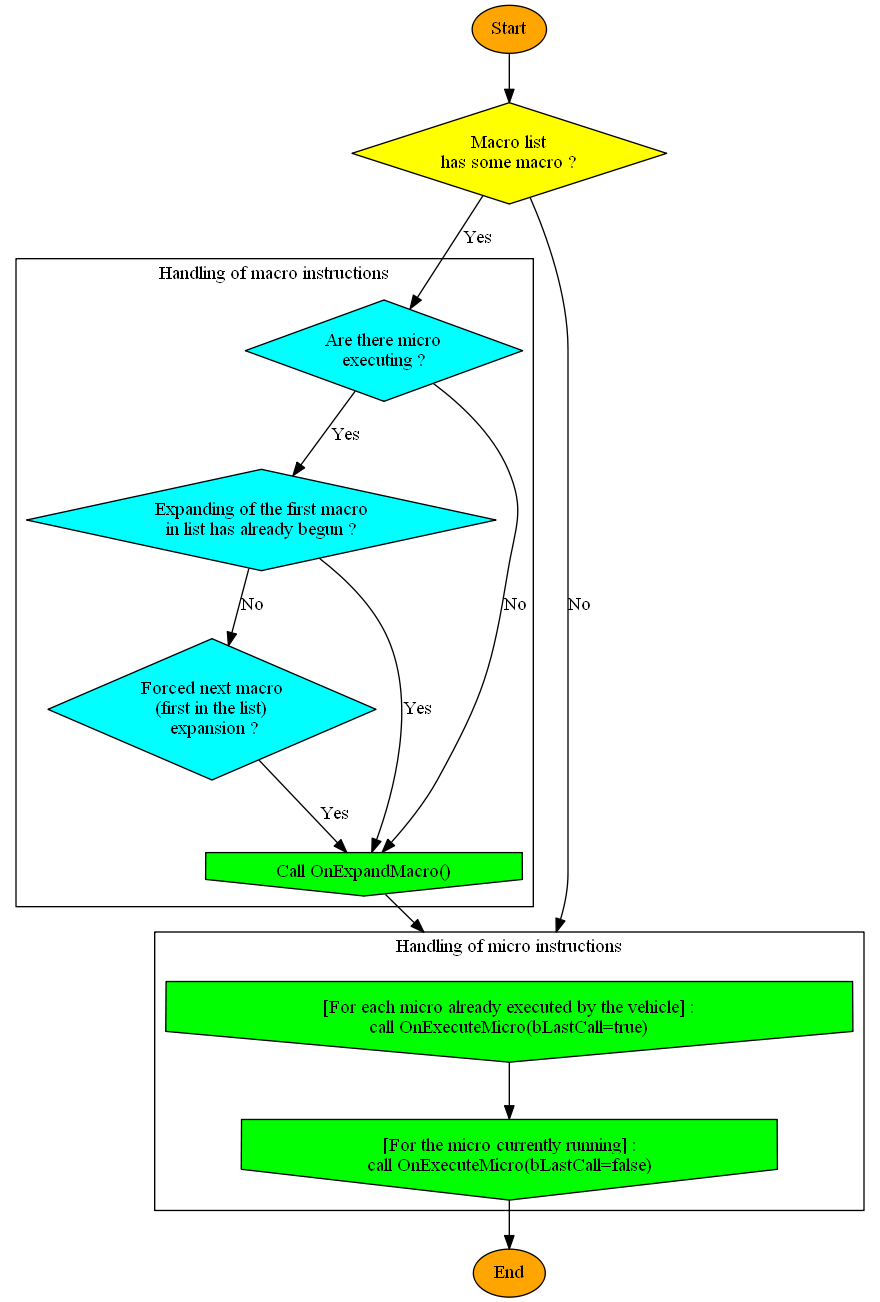
\includegraphics[scale=0.5]{agvmanager/missionExec}
	\caption{Main loop execution}
	\label{fig:missionExec}
\end{figure}

\section{Drag and drop example}
Let's consider a simple example. We have to write a script that react to mouse events from user. The vehicle have to move from one point to another.

First let's make a simple map, fig.\ref{fig:mapLine}, with one line $L_{1}$ and two generic points $P_{10}$ and $P_{20}$, the script will work on any map.
After the configuration with AgvConfigurator, we open AgvManager in order to write the script and simulate.
Notice that, after any modification of the script, AgvManager must be closed then opened.\\

\begin{figure}
	\centering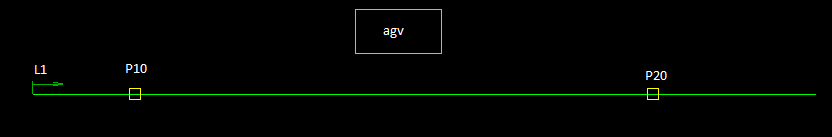
\includegraphics[scale=0.6]{agvmanager/agvManager/mapLine}
	\caption{Agv simple map, for drag and drop example. One line and two generic points.}
	\label{fig:mapLine}
\end{figure}

A simple program like this, should have at least the following callback functions:
\begin{enumerate}  
	\item OnApplicationStart() : bool 
	\item OnAgvDroppedToPoint(uint uAgv, uint uUser) 
	\item OnExpandMacro(uint uAgv, uint uMission, uint iMacroCode, int iPar1, int iPar2, int iPar3, int) : bool
	\item OnExecuteMicro(uint uAgv, bool bLastCall, int iMicroCode, int iPar0, int iPar1, int iPar2, int, int, int userId, int iMission, int) : bool
	\item OnAbortMission(uint uAgv)\\
\end{enumerate}

For simplicity we don't implement our own functions. Attached to this document will be provided the example we discuss here, and an equivalent example where other functions and files were added in order to keep the projects modular.
The modular example is organized as follow: 3 files, 5 callback functions, 2 user-defined functions and some variable and constant definitions.
A file called main.xs contain the inclusion of the other 2 files. A file called agvEventFunctions.xs where callback functions are implemented.
A file called common.xs where common functions and variables definitions are implemented. This strucutre is meant to be a template for future projects, as many functions can be reused. Of course other files and functions can be implemented. The structure of any project should be modular, portable and reusable.\\

The single file example have 5 callback functions and some constant definitions. By convention, constants are written using capital letters.
We will discuss the functions in order of execution. The function \textit{onAbortMission()} is called when a mission is aborted, it will be discussed at the end.

\subsubsection{onApplicationStart()}
The implementation of this function is shown in listing \ref{lbl_onApplicationStart}. As we say before, this is the first function called by agvManager.
first we create a variable \textit{mpar} of type \textit{XMapParms}. This is a structure that will contain informations about the vehicle.
By the function \textit{agvGetMapParams(xmapparams\&)} we read the existing data from AgvManager and we initialize the variable mpar with those data.
We change some parameter using the dot operator of the structure, for example we set the dimension of the vehicle i.e. \textit{mpar.setSymmetricalVehicleDimension(length, width)}. After we apply the changes to AgvManager using the function \textit{AgvSetMapParams(@mpar)}.

When the execution of this fucntion is done, AgvManager wait for some event. Let's suppose, the user drag the agv, in this case the event function \textit{OnAgvDroppedToPoint} is called.


\lstinputlisting[language=c++, firstline=107, lastline=147, caption=onApplicationStart implementation, label=lbl_onApplicationStart]{listing/agvDropToPoint_v0.xs}

\subsubsection{OnAgvDroppedToPoint(uint uAgv, uint uPointId) }
The call of this function is a response of mouse event. There are other mouse events like \textit{onAgvDroppedToLine()}.
In this function we set the behavior of the agv, what the agv have to do when it is dragged e.g. from $P_{10}$ and dropped to point $P_{20}$.
First let's put some requirements e.g. the agv should be in automatic mode, it should not be enabled, there is no mission in progress.
If those conditions are meeted the agv can move from one point to another. The code to control such conditions is self-explainatory in listing.\ref{lbl:OnAgvDroppedToPoint}.\\

This example will have only one mission, moving from one point to another. A mission should have at least one MACRO, every mission should have MAC\_END. This MACRO inform the manager that it reach the end of the mission.
There are some predefined constants for system used MACROs, they can be found in the documentation with the prefix MAC\_.
We can also define our own MACROs using the keyword Define. It is a good practice to use numbers from 100, every MACRO and mission should have a unique identifier.\\

Let's define our mission and a new MACRO:
\begin{lstlisting}[frame=single]
	; Mission null, ther is no mission
	$define MIS_NULL								0
	; Mission move to point
	$define MIS_TO_POINT						14
	
	; MACRO Movement to waypoint
	$define MAC_MOVE_TO_WP					100
\end{lstlisting}

In this case the mission MIS\_TO\_POINT is composed from 2 MACROs. In order the \textit{MACRO list} will have 2 elements:
\begin{enumerate}
	\item MAC\_MOVE\_TO\_WP
	\item MAC\_END \\
\end{enumerate}

Before starting a new mission we check if there is a mission in progress.
We call the function \textit{AgvActualMissionCode(uint uAgvId)}, this function return the id of the mission in progress.
If it return zero, it means there is no mission in progress. We have already define a constant MIS\_NULL as zero.
In the code we can write "\textit{if(AgvActualMissionCode(uAgv)=0)}", but it is always more readable when using names instead of numbers, so instead of 0 we use MIS\_NULL.\\

If there is no mission in progress, we can start the mission MIS\_TO\_POINT by calling the function \textit{bool AgvStartMission(uint uAgvId, uint CodeMissione, string sMissioneDescription)}, this function return true if the mission is in progress.

Now we have to fill the agv \underline{MACRO list} with our 2 MACROs, by calling the funntion \textit{bool agvAddMacro(uint uAgv,uint uCodeMACRO, int ipar1=0,int ipar2=0, int iapr3=0, int ipar4=0)}. The iparX have 0 as default value.

The first MACRO is MAC\_MOVE\_TO\_WP, this is a motion MACRO. So we have to build the path of the agv by calling the function AgvAddWaypoint(), this function take as parameters the agv id, the point id and direction and return an id of the point.

Then the MAC\_MOVE\_TO\_WP can be add to the list, by calling agvAddMacro(), giving it as ipar1 the return value of the function AgvAddWaypoint() and as ipar2 a flag to concatenate the execution of the next MACRO.
Then the macro MAC\_END that end our mission is add to the macro's list.

\begin{lstlisting}
	AgvStartMission(uAgv, MIS_TO_POINT, "Mission to point")
	;
	uint wpidx
	uchar destOrientation = 'X'
	bool concatenateNext = true
	;
	wpidx = AgvAddWaypoint(uAgv, uUser, destOrientation)
	AgvAddMacro(uAgv, MAC_MOVE_TO_WP, wpidx, concatenateNext)
	;
	AgvAddMacro(uAgv, MAC_END, MIS_TO_POINT)
\end{lstlisting}	


\lstinputlisting[language=c++, firstline=279, lastline=310, caption=OnAgvDroppedToPoint implementation. This function\, as input\, have the AGV id and the destination point id. This is an evznt function\, it is called when the user drag and drop the vehicle to the desired point, label=lbl:OnAgvDroppedToPoint]{listing/agvDropToPoint_v0.xs}

\subsubsection{OnExpandMacro()}
As we mentioned before, when a mission begin the function \textcolor{blue}{OnExpandMacro()} is called automatically by AgvManager. We already started a mission in the function  \textcolor{blue}{OnAgvDroppedToPoint()} and filled the MACRO list with 2 MACROs. So now we have to implement the function OnExpandMacro().

AgvManager executes the MACROs starting from the first one in the list. When it call the function \textcolor{blue}{OnExpandMacro()}, give it the \textcolor{red}{Agv id}, \textcolor{red}{mision id}, \textcolor{red}{MARCO code/id} and the four parameters stored in the list. We can imagine every elements of the list, is composed from those fields. So in the implementation of this function we check the MACRO code to be executed. We can use the case statement or the if in order to select our logic.

The first MACRO is MAC\_MOVE\_TO\_WP. Under the case MAC\_MOVE\_TO\_WP we implement the instructions to AgvManager:

\begin{lstlisting}
	case MAC_MOVE_TO_WP
		; iPar1 = Waypoint id
		; iPar2 = (bool) do concatenate next macro
			select (AgvMoveToWayPoint(uAgv, uMission, WpFl_RicalcolaPercorsi | WpFl_EliminaCompletato))
				case EsitoMov_MovimentoCompletato	; Completed movement
				case EsitoMov_RaggiuntoWaypoint		; Waypoint reached
					if (iPar2)
						AgvComputeNextMacro(uAgv)
					endif
					return true
				default
					return false
			endselect
		return true
\end{lstlisting}

In this code the motion instruction is done by calling \textcolor{blue}{AgvMoveToWayPoint()}, when this function return a value corresponding to \textcolor{blue}{MoveResult\_WaypointReached}, the next MACRO is expanded. The next MACRO in our example list is the \textcolor{blue}{END\_MACRO}.

\textit{When the return value of \textcolor{blue}{OnExpandMacro()} is \textcolor{red}{true}, it mean the current macro execution is terminate, and on the next call the following macro will be executed.} 

As we say every MACRO consist of different MICROs. A MACRO that correspond to a motion have a MIC\_MOVE. Here the MIC\_MOVE is registered by the call of the movement function \textit{AgvMoveToWayPoint()}.

The MAC\_END register a MIC\_SYSTEM micro type. When the MAC\_END is expanded, it start or register a new micro. Simply this MACRO have only one MIC\_SYSTEM micro type that is S\_END.

This MICRO inform AgvManager that the mission is ended. In the case MAC\_END the micro S\_END is registered by calling \textit{AgvRegisterSystemBloccante(uAgv, uMission, S\_END)}, where the function \textit{agvStopMission(uagv)} is called, as we will see in the function \textit{onExecuteMicro()}.\\

As shown in fig.\ref{fig:missionExec}, AgvManager continue to call onExpandMacro() and onExcecuteMicro().

When the \textcolor{blue}{onExpandMacro()} terminate the function onExcecuteMicro() is called.\\

In the tab \textcolor{red}{vehicle informations[F3]}, under Agv commands we can se a list of missions, macros expansion and micro instructions, as well as information about them, fig.\ref{fig:macro_expansion_1}, fig.\ref{fig:macro_expansion_2} and fig.\ref{fig:macro_expansion_3}.\\

\begin{figure}
	\centering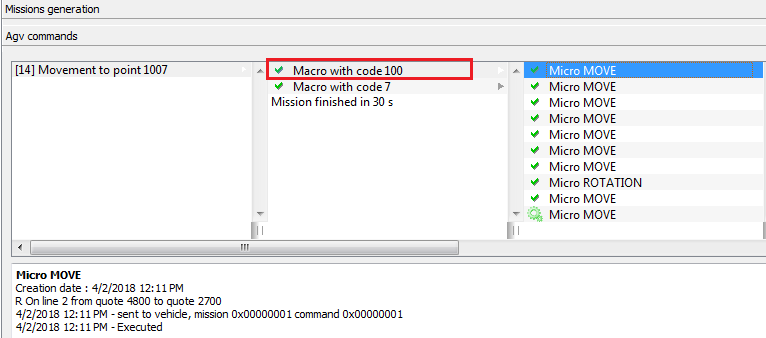
\includegraphics[scale=0.7]{agvmanager/agvManager/macro_expansion_1}
	\caption{Movment to point 1007, Macro MAC\_MOVE\_TO\_WP=100. As we can see, the macro consist of a list MICROs. Selecting a mission or a macro or a micro we can see informations about them.}
	\label{fig:macro_expansion_1}
\end{figure}
\begin{figure}
	\centering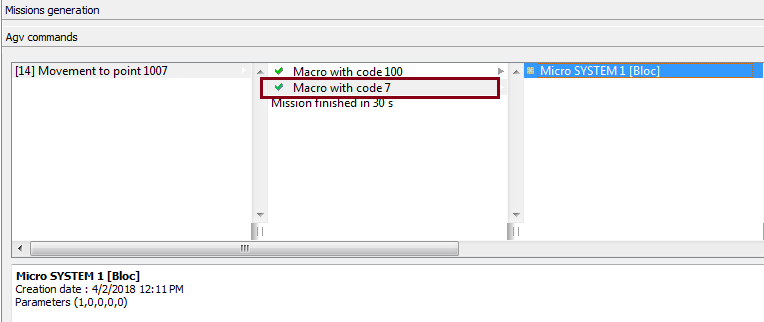
\includegraphics[scale=0.7]{agvmanager/agvManager/macro_expansion_2}
	\caption{Movement to point 1007, Macro MAC\_END=7. As we can see, the macro consist of on system micro that is S\_END.}
	\label{fig:macro_expansion_2}
\end{figure}
\begin{figure}
	\centering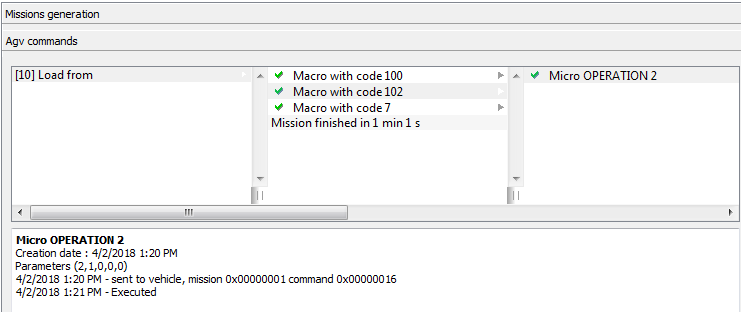
\includegraphics[scale=0.7]{agvmanager/agvManager/macro_expansion_3}
	\caption{Mission load from a user point. The macro expansion shows 3 macros in the list. The MACRO 102, user defined, have only one micro of type operation that is O\_LOAD, system defined. Later we will the commands sent to agv in order to execute operations.}
	\label{fig:macro_expansion_3}
\end{figure}

\lstinputlisting[language=c++, firstline=170, lastline=215, caption=OnExpandMacro, label=lbl:OnExpandMacro]{listing/agvDropToPoint_v0.xs}

\subsubsection{OnExecuteMicro()}

MICROs are instructions to the vehicle. MICROs are stored in a list, one MACRO can register more than one MICRO fig.\ref{fig:macro_expansion_1}.

For example a MICRO can be registered by calling \textcolor{blue}{agvRegisterSystemBloccante()} or  \textcolor{blue}{agvRegisterSystemPassante()} for MIC\_SYSTEM type or \textcolor{blue}{AgvRegisterOperation()} for MIC\_OPERATION type. See documentation for a more complete list of micro registration functions.
These function have uAgv, uMission, MICROcode as input parameters.

There are different types of MICROs, that can be found in the documentation with prefix MIC\_. Let's see MIC\_SYSTEM to which the S\_END belong, this type of MICRO doesn't send any instruction to the agv itself. For example S\_END is need to end a mission, and is managed by AgvManager.\\

For example listing.\ref{lstRegisterSystem}, register a 30 seconds waiting time.

\begin{lstlisting}[caption=Wait time system micro ,label=lstRegisterSystem]
	$define S_START_WAIT				100
	$define S_EXEC_WAIT					101
	AgvRegisterSystemBloccante(uAgv, uMission, S_START_WAIT, iPar1)
	AgvRegisterSystemBloccante(uAgv, uMission, S_EXEC_WAIT)
\end{lstlisting}
	

A MIC\_MOVE type is related to instruction of motion sent to the agv. A MIC\_OPERATION is an operation like loading and unloading. \\

There are 2 kinds of micros: blocking and non-blocking MICROs. The difference is that the blocking MICRO lock the execution of other micros till the end of the execution of itself or till the verification of a condition. \\

When expanding macros, the micro list is composed by calling the relative registration function.
For example, in the function \textcolor{blue}{OnExpandMacro()} under the MAC\_END, we register a blocking system micro, S\_END.
In the function \textcolor{blue}{onExecuteMicro()} under the case MIC\_SYSTEM and under the case S\_END we call the function \textcolor{blue}{AgvStopMission(uAgv)} in order to stop the mission. When a micro terminate the execution of the function \textcolor{blue}{onExecuteMicro()} return true. \\

When the mission is stopped the macro list is eliminated, and the agv is ready to get another mission. 

\lstinputlisting[language=c++, firstline=217, lastline=277, caption=OnExecuteMicro, label=lbl:OnExecuteMicro]{listing/agvDropToPoint_v0.xs}

\section{Summary}
In automatic mode, if the Agv is not executing a mission, if it is enabled the callback function \textcolor{blue}{onNextMission()} is called. If there is a mission in progress, even if the Agv is not enabled, continue to execute the mission till the end or till receiving an abort mission command, see fig.\ref{fig:mainLoop}.

For example, in the implementation of the function \textcolor{blue}{onNextMission()} missions can be assigned to agv depending on the plant status, e.g. by calling a user defined function \textcolor{blue}{RegisterMission()}. Th signature of the the function \textcolor{blue}{RegisterMission()} can be defined as we wish.

\begin{lstlisting}[caption=onNextMission() missions are assigned]
	//onNextMission()
	
	// register mission depending on the plant logic
	RegisterMission(uAgv, MIS\_LOAD\_FROM\_STATION, iPar1, iPar2)
\end{lstlisting}

In the function \textcolor{blue}{RegisterMission()}, depending on the mission we compile the \textcolor{red}{macro list}. For example if our mission is to go to load a product the macro list will composed in the following way:
\begin{lstlisting}[caption=RegisterMission() macro list is composed]
	// RegisterMission()
	
	//Start mission with id uMissionCode
	AgvStartMission(uAgv, uMissionCode, MissionDescription)

	case MIS_LOAD_FROM_STATION
		//
		uint wpidx
		uchar destOrientation='X'
		bool concatenateNext=true
		wpidx = AgvAddWaypoint(uAgv, ID_LOAD_STATION, destOrientation)
		AgvAddMacro(uAgv, MAC_MOVE_TO_WP, wpidx, concatenateNext)
		
		// Wait for operator to load toilet
		AgvAddMacro(uAgv, MAC_WAIT_END_LOADING)
		
		// END of this mission
		AgvAddMacro(uAgv, MAC_END, uCode)
		break
\end{lstlisting}

When a mission is in progress, and the macro list is not empty, the callback function \textcolor{blue}{onExpandMacro()} is called. Depending on the macro we compile a list of micro instructions. For example one of the macros was \textcolor{blue}{MAC\_WAIT\_END\_LOADING}:

\begin{lstlisting}[caption= onExpandMacro() micro list is composed]
	//onExpandMacro()
	case MAC_WAIT_END_LOADING
		AgvRegisterSystemBloccante(uAgv, uMission, S_START_WAIT, 30)
		AgvRegisterSystemBloccante(uAgv, uMission, S_EXEC_WAIT)
		AgvRegisterOperation(uAgv, uMission, O_WAIT_LOAD)
		break
\end{lstlisting}

After the call of \textcolor{blue}{onExpandMacro()} the callback function \textcolor{blue}{onExecuteMicro()} is called, and depending on the micro we execute operation and instructions:

\begin{lstlisting}[caption=onExecuteMicro() micro are aexecuted]
	//onExecuteMicro()
	
	case S_START_WAIT
		timerWait[uAgv] = timeoutS(iPar1)
		break
	
	case S_EXEC_WAIT
		if (isTimeout(timerWait[uAgv]))
			return true
		else
			MultiMessageState(uAgv, "Agv " + (uAgv + 1) + " : wait " + int(secsToTimeout(timerWait[uAgv])) + "s")
			return false
		endif
		break
\end{lstlisting}

The state of mission execution is monitored cyclically. This mean that when a mission begin the functions \textcolor{blue}{onExpandMacro()} and \textcolor{blue}{onExecuteMicro()} are called repeatedly until the end of the mission, see fig. \ref{fig:missionExec}.
The \textcolor{blue}{onExpandMacro()} start executing the following macro in the list, when the previous returned true. The following micro is executed when \textcolor{blue}{onExecuteMicro()} return true. the flag \textcolor{red}{bLastCall} is set to true by agvManager.

The main logic of AGVs is written in the function \textcolor{blue}{onNextMission()}, where missions are assigned to AGV. When the logic is divided by missions, it is relatively easy to write the other 3 main functions : \textcolor{blue}{ registerMission(), onExpandMacro() and onExecuteMicro()}. Helper functions can be implemented to implement some useful logic.